\section{Introducation}
Mobile systems have clear requirements for user satisfaction: they
must meet performance goals necessary for interacting with sensors and
human users and must conserve energy to maximize battery life.  To
address these conflicting requirements, hardware platforms have become
increasingly diverse.  Many mobile processors support, for example,
different core types with different performance/power tradeoffs, which
can be operated at many different speeds.  Meeting performance
requirements is further complicated by the dynamic nature of computing
systems: application resource demands can vary widely as a function of
input or application phase and multiple applications may compete for
resources.

\begin{figure}
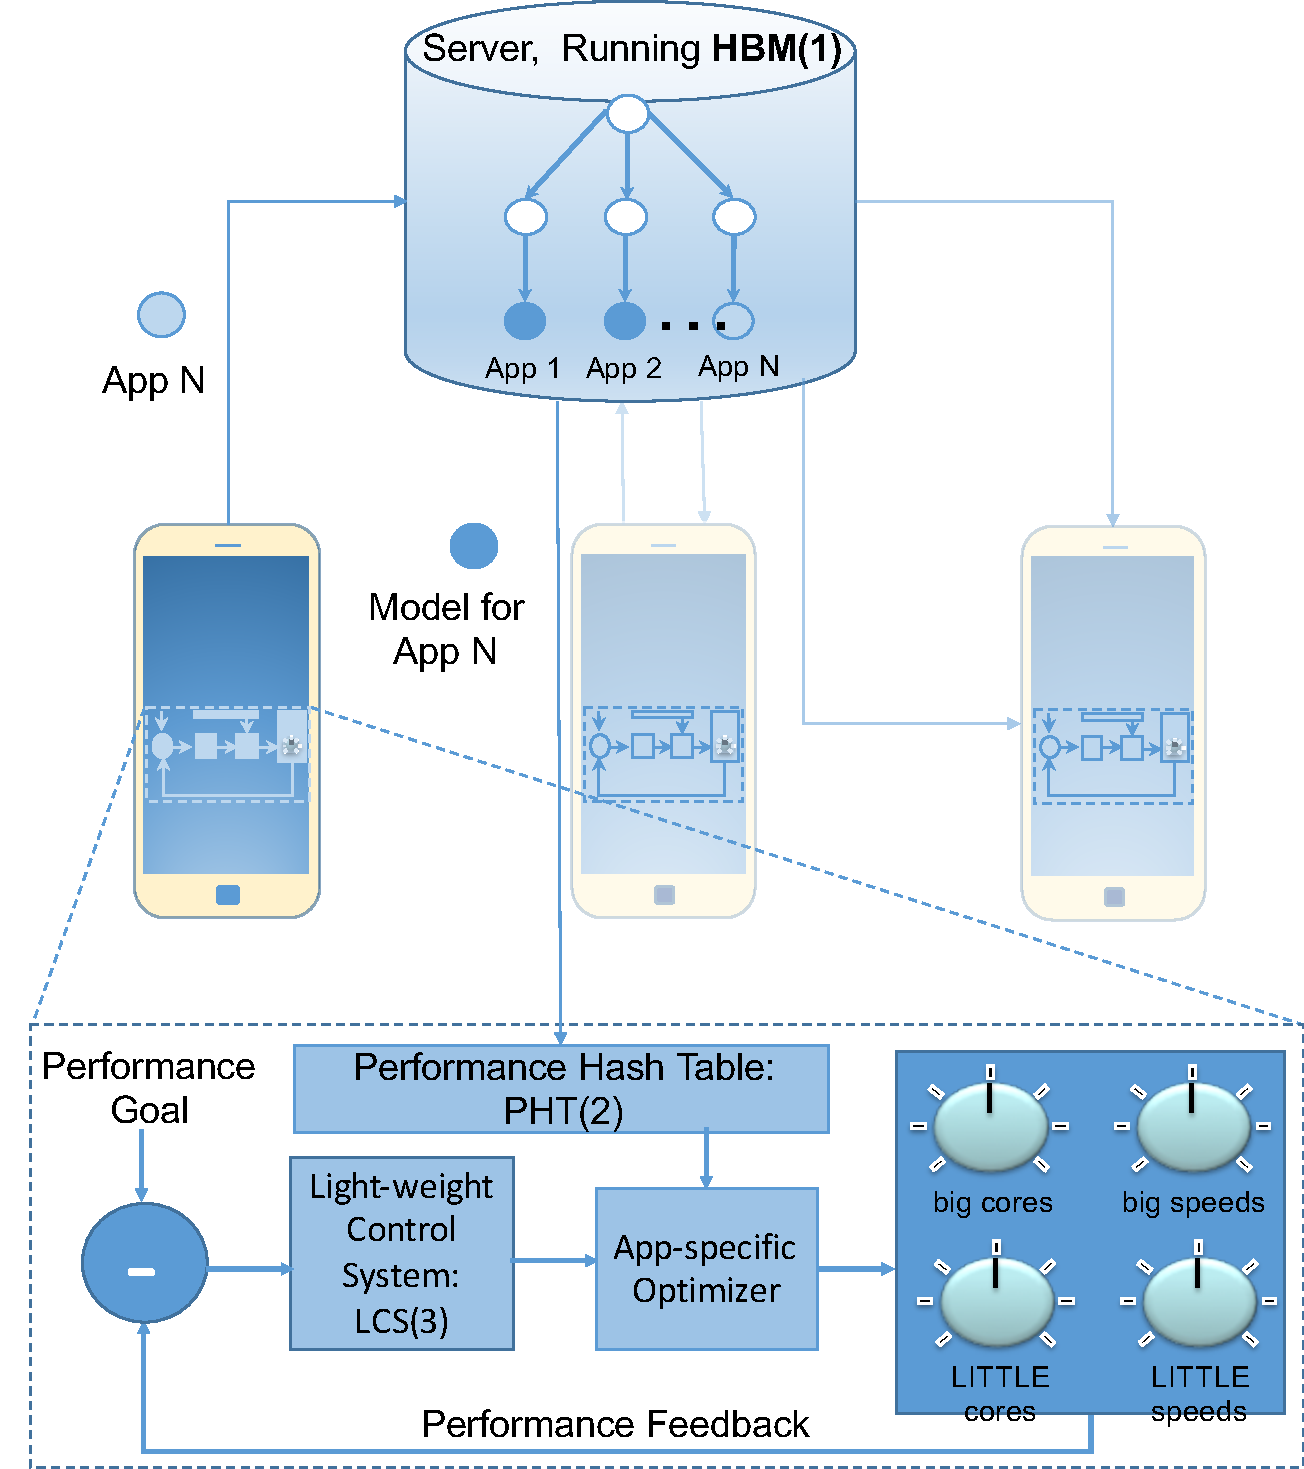
\includegraphics[width=\columnwidth]{figures/mobile-leo-poet.pdf}
\caption{\SYSTEM{} overview.}
  \label{fig:overview}
\end{figure}

Thus, two central challenges arise to meeting performance requirements
with minimal energy on mobile systems: (1) complexity and (2)
dynamics.  Each challenge has been addressed individually.  First,
machine learning approaches can model the complicated,
power/performance tradeoff spaces that arise on configurable,
heterogeneous mobile systems
\cite{dubach2010,Bitirgen2008,Ipek,Koala,LEO,Flicker,Ponamarev}.  Such
approaches can learn complex models, identifying and avoiding local
extrema that lead to inefficient resource usage.  Second, control
theoretic techniques ensure performance is met with minimal energy by
tuning resource allocation using application feedback
\cite{Wu2004,Chen2011,PTRADE,POET,ControlWare,Agilos,grace2}.  Control
techniques provide a formal basis for reasoning about dynamics and can
ensure performance requirements are met despite application, input, or
workload fluctuations.

Learning and control techniques have complementary strengths and
weaknesses.  Learning approaches handle complexity -- including
non-linearities and non-convexity -- but have no established mechanism
for managing system dynamics.  Control approaches handle dynamics, but
rely on linear models that are increasingly insufficient to capture
the diversity of modern hardware.

We therefore propose combining learning and control techniques to
manage both complexity and dynamics.  We call our approach
\SYSTEM{}\footnote{\textbf{C}ontrol \textbf{A}nd \textbf{L}earning for
  \textbf{O}ptimal \textbf{R}esource \textbf{E}nergy
  \textbf{E}fficiency} and it has three components as illustrated in
\figref{overview}: (1) a hierarchical Bayesian model (HBM) that learns
application-specific relationships between performance/power and
resource usage, (2) a lightweight control system (LCS) that
dynamically tunes resource usage to meet performance requirements with
minimal energy, and (3) a performance hash table (PHT) that serves as
the interface between learning and control.  The HBM produces accurate
models of power and performance, but it is computationally expensive,
so in \SYSTEM{} the HBM runs on a remote server.  As it is remote, it
is also capable of aggregating data from multiple devices.  The LCS
runs on individual mobile devices and receives models from the HBM.
These models are stored in the PHT, a data structure that allows the
LCS to determine energy minimal resource schedules in constant time.


The PHT is \SYSTEM{}'s key enabler.  While learning and control
systems exist, their combination requires an appropriate interface.
The challenge is that the learner produces non-linear models of
discrete resources (\eg cores and clockspeeds), while the control
system is based on continuous linear models.  \SYSTEM{} bridges this
gap by scheduling resources in time to meet a performance requirement
with minimal energy.  The PHT stores the learned models in such a way
that this optimization problem can be solved in constant time, making
it appropriate for use on a mobile device.  While only tested with
\SYSTEM{} we believe the PHT is general enough to be used by different
learning and control systems, or even to solve different optimization
problems.


% While control and learning frameworks exist, the key to combining them
% is creating an interface between the learning and control systems.
% Specifically, learning frameworks for resource management map
% configurations (\eg resource allocations) into estimated performance
% and power.  These mappings are discrete and non-linear, capturing the
% behavior of the underlying system.  Controllers, in contrast, work
% with continuous linear models.  Therefore, our proposed combination of
% learning and control requires an interface to convert the discrete
% non-linear learned models into continuous linear models.  We address
% this challenge by forming the lower convex hull of points on the
% learned power/performance tradeoff space.  Interpolating between these
% points gives us a piecewise linear function that is appropriate for
% control models, yet still captures the significant behavior of the
% underlying system.  This interface allows us to combine the approaches
% studied in this paper, and we believe it is sufficiently general to
% apply to other combinations of learning and control as well.

We test \SYSTEM{} on ARM big.LITTLE platforms with 20 different
benchmarks to evaluate the HBM's ability to learn application specific
models and the LCS's ability to deliver performance efficiently.  We
compare to published learning and control methods in a variety of
settings.  While many applications have inherent dynamics (\ie
different processing phases), we explicitly test the ability to adapt
to the unknown by running each application with other, random
applications.  We evaluate both the ability to meet performance
requests and minimize energy consumption.  We find that \SYSTEM{}:
\TODO{Double check all the numbers once we have the final values from
  the evaluation section.}
\begin{itemize}
\item \textbf{Delivers Reliable Performance: } We calculate the error
  between the desired and delivered performance.  When running one
  application at a time, \SYSTEM{} achieves an average error of 2.1\%,
  compared to 3.4-5.4\% for existing learning methods and 4.6\% for
  existing control approaches.
\item \textbf{Uses Lower Average Energy:} We compare energy
  consumption to the optimal found through exhaustive search.  When
  running one application at a time, \SYSTEM{} achieves an average
  energy consumption of 7\%, greater than optimal compared to 25-52\%
  for existing learning methods and 26\% for existing control
  approaches.
\item \textbf{Provides Better Worst Case Behavior:} In the single
  application case, \SYSTEM{} worst observed error across all
  applications and targets is 9\% compared to 19-73\% for prior
  learning methods and 25\% for existing control methods.  The worst
  observed energy for \SYSTEM{} is 1.82$\times$ greater than optimal,
  while it is 4-12$\times$ greater for learning and 2.9 $\times$
  greater for control.
\item \textbf{Adapts to Dynamics:} We test \SYSTEM{}'s ability to deal
  with changing environments by running each benchmark with a
  performance target and then randomly starting another application on
  one core.  Even though the available resources fluctuate
  dynamically, \SYSTEM{}'s worst performance error is 30\%, while it
  is 71-84\% for prior learning approaches and 35\% for prior control
  approaches.  Additional studies show \SYSTEM{} reacting to input
  changes and application behavioral changes.
\end{itemize}
In summary, this paper makes the following contributions:
\begin{itemize}
\item Proposing the combination of a hierarchical Bayesian learning
  with a lightweight control system to meet the twin challenges of
  addressing complexity and dynamics to deliver performance with
  minimal energy on mobile systems.
\item An interface for combining discrete learned models of resource
  usage with continuous control models of resource dynamics.
\item Evaluating the implementation and comparison to existing,
  independent learning and control techniques.
\end{itemize}


